%% 
%% Copyright 2019-2024 Elsevier Ltd
%% 
%% This file is part of the 'CAS Bundle'.
%% --------------------------------------
%% 
%% It may be distributed under the conditions of the LaTeX Project Public
%% License, either version 1.3c of this license or (at your option) any
%% later version.  The latest version of this license is in
%%    http://www.latex-project.org/lppl.txt
%% and version 1.3c or later is part of all distributions of LaTeX
%% version 1999/12/01 or later.
%% 
%% The list of all files belonging to the 'CAS Bundle' is
%% given in the file `manifest.txt'.
%% 
%% Template article for cas-dc documentclass for 
%% double column output.

\documentclass[a4paper,fleqn]{cas-dc}


\newcommand{\fb}{\color{blue}}
\newcommand{\mt}{\color{red}}
\newcommand{\al}{\color{ForestGreen}}

% If the frontmatter runs over more than one page
% use the longmktitle option.

%\documentclass[a4paper,fleqn,longmktitle]{cas-dc}

%\usepackage[numbers]{natbib}
%\usepackage[authoryear]{natbib}
\usepackage[authoryear,longnamesfirst]{natbib}
\usepackage{cuted}
\usepackage{csquotes}
\usepackage{tikz}
\usetikzlibrary{arrows.meta}


\usepackage{gensymb}
%%%%%%%%%%%%%%%%%%%%TODO
\usepackage[colorinlistoftodos]{todonotes}
\let\xtodo\todo
\renewcommand{\todo}[1]{\xtodo[inline,color=black!5]{#1}}



%%%Author macros
\def\tsc#1{\csdef{#1}{\textsc{\lowercase{#1}}\xspace}}
\tsc{WGM}
\tsc{QE}
%%%

\DeclareMathOperator*{\argmin}{arg\,min}

% Uncomment and use as if needed
%\newtheorem{theorem}{Theorem}
%\newtheorem{lemma}[theorem]{Lemma}
%\newdefinition{rmk}{Remark}
%\newproof{pf}{Proof}
%\newproof{pot}{Proof of Theorem \ref{thm}}

\begin{document}
\let\WriteBookmarks\relax
\def\floatpagepagefraction{1}
\def\textpagefraction{.001}

% Short title
\shorttitle{}    

% Short author
\shortauthors{Frank Bastian, Mohit Tunwal, and Aaron Lim}  

% Main title of the paper
\title [mode = title]{
InfoMag: Downward continuing INFOMAR's magnetometry data
} 


% Title footnote mark
% eg: \tnotemark[1]
\tnotemark[1] 

% Title footnote 1.
% eg: \tnotetext[1]{Title footnote text}
\tnotetext[1]{} 

% First author
%
% Options: Use if required
% eg: \author[1,3]{Author Name}[type=editor,
%       style=chinese,
%       auid=000,
%       bioid=1,
%       prefix=Sir,
%       orcid=0000-0000-0000-0000,
%       facebook=<facebook id>,
%       twitter=<twitter id>,
%       linkedin=<linkedin id>,
%       gplus=<gplus id>]

\author[1]{Frank Bastian}%[<options>]
\author[2]{Mohit Tunwal}
\author[3]{Aaron Lim}

% Corresponding author indication
\cormark[1]

% Footnote of the first author
\fnmark[1]

% Email id of the first author
\ead{}

% URL of the first author
\ead[url]{}

% Credit authorship
% eg: \credit{Conceptualization of this study, Methodology, Software}
\credit{}

% Address/affiliation
\affiliation[1]{organization={},
            addressline={}, 
            city={},
%          citysep={}, % Uncomment if no comma needed between city and postcode
            postcode={}, 
            state={},
            country={}}

%\author[2]{}%[]

% Footnote of the second author
%\fnmark[2]

% Email id of the second author
%\ead{}

% URL of the second author
\ead[url]{}

% Credit authorship
\credit{}

% Address/affiliation
\affiliation[2]{organization={},
            addressline={}, 
            city={},
%          citysep={}, % Uncomment if no comma needed between city and postcode
            postcode={}, 
            state={},
            country={}}

% Corresponding author text
\cortext[1]{Corresponding author}

% Footnote text
\fntext[1]{}

% For a title note without a number/mark
%\nonumnote{}

% Here goes the abstract
\begin{abstract}
The {\al INFOMAR} programme {\al is Ireland’s national seabed mapping programme that maps the country’s marine territory to support sustainable development, environmental protection, and marine resource management}.  {\al over} the last 20 years various geological data sets such as bathymetry, sub-bottom profiler, or magnetometry data {\al have} been {\al acquired} {\al with significant portions of the bathymetry and backscatter data processed and made publicly available}. However this has not been the case for the magnetometry data {\al which remains largely unprocessed in its raw format}. Here, we present an{\mt (how about free and open source?)} open-source graphical user interface {\al (GUI)}{\mt, built on python environment, }that can process {\al these} data set and enables {\al subsequent analysis through} its exported {\al magnetic} anomaly grids.
{\al Given that the INFOMAR magnetometry data are uniquely surface-acquired,} the software implements an iterative algorithm to downward continue the surface-acquired field to the seabed using bathymetry data to {\al help align with best practice}. {\mt The software presented here will open up the avenue to process and unlock the potential of magnetometry data beyond Irish shelf.}

\end{abstract}

% Use if graphical abstract is present
%\begin{graphicalabstract}
%\includegraphics{}
%\end{graphicalabstract}

% Research highlights
\begin{highlights}
\item 
\item 
\item 
\end{highlights}


%\nocite{*}

% Keywords
% Each keyword is seperated by \sep
\begin{keywords}
Infomar \sep Magnetic anomaly \sep Downward continuation \sep
\end{keywords}

\maketitle

% Main text
\section{Introduction}\label{}


{\mt Adding an outline of Introduction - 
Para 1 - Broadest intro opening: Things to mention

- How is mag data collected and processed? Why is magnetometry data important?


Para 2 - Discuss issue 1:
- Challenges in processing mag data?
- Cost? SKill? 
- How much data Irish and possibly other surveys are sitting on? Commercial/academic implications?

Para 3 - Discuss issue 2:
- Even with process data, raw survey data is collected at different depths
- Challenges related to it?
- Current ways of tackling it?

Para 4 - You are lord and saviour of mag world by solving the above two issues:

- In this paper we present..

-The aim of this paper/software is to ...

-Finally paper outline

Feel free to add on to above, I will add fair text as we go along
}


The Integrated Mapping for the Sustainable Development of Ireland's Marine Resource (Infomar) programme\footnote{\url{https://www.Infomar.ie/}} is a joint initiative between the Marine Institute (MI) and the Geological Survey of Ireland (GSI) to survey and map the entirety of Ireland's seafloor territory. Until today, the programme has collected data sets on bathymetry, sub-bottom profiles, shipwrecks and magnetometry. 

However, the magnetometry data set remained untouched mostly due to the fact that it had been surface acquired.
Here, we present a software enabling end-users to process this data set.
This includes preprocessing, the visualisation, and export of anomaly grids.
Using the processed bathymetry data sets, the software can continue the magnetometry data set downward to the seabed.

The paper consists of two parts.
First, we establish in Sec.~\ref{sec:Theory} the theoretical background of downward continuation.
Subsequent in Sec.~\ref{sec:Software}, we present the software that implements a processing pipeline including an optional downward continuation of the Infomar data set.

\todo{Not happy how the the introduction reads}




\section{Theory}\label{sec:Theory}
Following \cite{blakely1996potential,henderson1970validity}, we denote $\bar{B}$ as the Earth's normal total magnetic field intensity vector, assumed to be uniform across the region and $b$ to represent the unit vector in the direction of $\bar{B}$.
Additionally, we denote $B$ as the total magnetic intensity vector, whose magnitude $\lvert B\rvert$ is measured by the magnetometer.
The presence of ferromagnetic materials, e.g. iron, gives rise to an \todo{double check and find citation}
anomalous vector is $\Bar{B}-B$ and the anomaly value $U$:
\begin{equation}
	U = (\Bar{B}-B) \cdot b.
	\label{eq:trueAnomaly}
\end{equation}
Following the standard assumption of $U\ll \bar{B}$, we approximate the {\bf total field magnetic anomalies}:
\begin{equation}
	U(x,y,z_0) = \lvert\Bar{B}\rvert-\lvert B\rvert,
	\label{eq:anomalies}
\end{equation}
since a standard magnetometer does not obtain the direction of $B$~\cite{henderson1970validity}. 

%Consider a continuous function $U$, with continuous derivatives that is harmonic ($\nabla^2 =0$), in a regular region $R$.
% From Green's third identity, we have that the value of $U$ at any point $P$ within $R$ is given by 
% \begin{equation}
	%     U(P) = \frac{1}{4\pi}\int_{S} \left( \frac{1}{r} \frac{\partial U}{\partial n}-U\frac{\partial}{\partial n}\frac{1}{r}\right) dS,
	% \end{equation}
% where $S$ is denotes the boundary of $R$, $n$ the outward normal direction, and $r$ the distance from $P$ to the point of integration on $S$.

Using a Cartesian coordinate system where the z-axis is directed upward, we denote the total magnetic field at sea level $z_0$ as $U(x', y', z_0)$.
We are interested in the total magnetic field at the seabed, i.e. $z  = z_0 + \Delta  z$, with $\Delta z<0$, given as
\begin{equation}
	\begin{split}
		&U(x,y,\Delta z)\\
		=& \frac{-\Delta z}{2\pi} \int_{-\infty}^{\infty}\int_{-\infty}^{\infty} \frac{U(x', y', z_0)}{\left[(x-x')^2+(y-y')^2+\Delta  z^2\right]^{3/2}} dx' dy'.
		\label{eq:keyIntegral}
	\end{split}
\end{equation}
We note that Eq.~\eqref{eq:keyIntegral} is indeed a two-dimensional convolution,
\begin{equation}
	\begin{split}
		&U(x,y,\Delta  z) \\
		=& \int_{-\infty}^{\infty}\int_{-\infty}^{\infty} U(x', y', z_0) \psi(x-x',y-y',\Delta  z) dx'dy',
		\label{eq:convolutionAsIntegrals}
	\end{split}
\end{equation}
where
\begin{equation}
	\psi (x,y,\Delta  z) = \frac{-\Delta  z}{2\pi} \frac{1}{(x^2+y^2+\Delta  z^2)^{3/2}},
	\label{eq:psi}
\end{equation}
and seek to apply the Fourier-convolution theorem.
Or in other words, we rewrite Eq.~\eqref{eq:convolutionAsIntegrals} as
\begin{equation}
	\mathcal{F}[U(x,y,\Delta z)] = \mathcal{F}[U(x',y',z_0)]\mathcal{F}[\psi(x,y,\Delta z)].
	\label{eq:up_or_down_theory}
\end{equation}
Here, $\mathcal{F}[U(x',y',z_0)]$ denotes the Fourier transform of total magnetic field $U(x,y,z_0)$ measured on the surface $z = z_0$ given as
\begin{equation}
	\begin{split}
		&\mathcal{F}[U(x',y',z_0)](u,v)\\
		= &\int_{-\infty}^{\infty}\int_{-\infty}^{\infty} U(x',y',z_0) e^{-i(ux+vy)} dx'dy',
	\end{split}
	\label{eq:FourierTransform}
\end{equation}
with its inverse transformation given as
\begin{equation}
	\begin{split}
		&\mathcal{F}^{-1}[\mathcal{F}[U(u,v)]\\
		=&\frac{1}{2\pi}\int_{-\infty}^{\infty}\int_{-\infty}^{\infty}\mathcal{F}[U(u,v)e^{i(ux+vy)} dudv,
	\end{split}
\end{equation}
and $\mathcal{F}[\psi(x,y,\Delta z)]$ denoting the Fourier transform of Eq.~\eqref{eq:psi} given by
\begin{equation}
	\mathcal{F}[\psi(x,y,\Delta z)] = e^{-\Delta z \sqrt{u^2+v^2}}.
	\label{eq:Fpsi}
\end{equation}
Accordingly, the field $U(x,y,\Delta z)$ can be obtained by transforming Eq.~\eqref{eq:up_or_down_theory} back into the special domain:  
\begin{equation}
	\begin{split}
		%&\mathcal{F}^{-1}[\mathcal{F}[U(x,y,z_0)]] =\\
		&U(x,y,\Delta z)\\
		=& \frac{1}{4\pi^2} \int_{-\infty}^{\infty}\int_{-\infty}^{\infty} \mathcal{F}[U(x',y',z_0)](u,v) e^{-\Delta z\sqrt{u^2+v^2}+i(ux+vy)} dudv.
	\end{split}
	\label{eq:inverseFourierTransfor}
\end{equation}
% Using Eq.\eqref{eq:FourierTransform}, we can rewrite Eq.~\eqref{eq:convolutionAsIntegrals}:
% \begin{equation}
	%     \mathcal{F}[U(x,y,z)] = \mathcal{F}[U(x,y,z_0)]\mathcal{F}[\psi(x,y,z)],
	%     \label{eq:up_or_down_theory}
	% \end{equation}
% and $\mathcal{F}[U(x,y,z)]$ denoting the Fourier transform of the continued field and $\mathcal{F}[\psi]$ denoting the Fourier transform of Eq.~\eqref{eq:psi} given by
% \begin{equation}
	%     \mathcal{F}[\psi] = e^{-z \sqrt{u^2+v^2}}.
	%     \label{eq:Fpsi}
	% \end{equation}
Here, $\Delta z > 0$ denotes an uplifting and smoothing of the data.
However, we are interested in $\Delta z < 0$, i.e. downlifting it to the seabed.
As indicated in Eq.~\eqref{eq:Fpsi}, this corresponds to an exponential amplification of high frequencies, rendering a naive approach numerically very unstable~\cite{blakely1996potential}.
To overcome this, various methods using different techniques, such as Tikhonov regularization~\cite{RREGCONT_Tikhonov} or neural networks~\cite{}, have been proposed.

We follow \cite{stable_downward_iterative} that presented an iterative method of calculating the downward continued field based on the Taylor expansion
\begin{equation}
	\begin{split}
		&U(x,y, z)\\
		=& U(x,y,z_0) + \frac{\partial U(x,y,z_0) }{\partial z} z + \frac{1}{2!}\frac{\partial^2U(x,y,z_0)}{\partial z^2} z^2
		+\dots,
	\end{split}
	\label{eq:key_taylor}
\end{equation}
$z = \Delta  z>0$ denoting an uplifting and $z = -\Delta z <0$ denoting a downlifting.

The key idea, now is to use the upward continued field $U(x,y,\Delta z)$ since upward continuing is a stable operation.
The Taylor expansion of $U(x,y,\Delta z)$ is given as:
\begin{equation}
	\begin{split}
		&U(x,y,\Delta z),\\
		=& U(x,y,z_0) + \frac{\partial U(x,y,z_0) }{\partial z}\Delta  z + \frac{1}{2!}\frac{\partial^2 U(x,y,z_0)}{\partial z^2}\Delta  z^2+\dots
	\end{split}
	\label{eq:taylor_up}
\end{equation}
and accordingly the Taylor expansion of the downward field $U(x,y,-\Delta z)$ is given as:
\begin{equation}
	\begin{split}
		&U(x,y,-\Delta z),\\
		=& U(x,y,z_0) - \frac{\partial U(x,y,z_0) }{\partial z}\Delta  z + \frac{1}{2!}\frac{\partial^2 U(x,y,z_0)}{\partial z^2}\Delta  z^2+\dots
	\end{split}
	\label{eq:taylor_down}
\end{equation}

Adding Eq.~\eqref{eq:taylor_up} with Eq.~\eqref{eq:taylor_down} and rearranging gives,
\begin{equation}
	U(x,y,-\Delta  z) = 2 U(x,y,z_0) - U(x,y,\Delta  z) + \frac{\partial^2U(x,y,z_0)}{\partial z^2}\Delta  z^2
	\label{eq:Taylor_sum}
\end{equation}
Since $U(x,y,\Delta  z)$ can be obtained through Eq.~\eqref{eq:inverseFourierTransfor}, the only thing left is to calculate the second-order vertical derivate
\begin{equation}
	\frac{\partial^2U(x,y,z_0)}{\partial z^2}
	= -\left(\frac{\partial^2 U (x,y,z_0)}{\partial x^2} +\frac{\partial^2 U(x,y,z_0)}{\partial y^2} \right),
\end{equation}
Here, we deviate from \cite{stable_downward_iterative}, who calculated the second-order vertical derivative in special domain.
Instead, we estimate the vertical derivative in spectral domain
\begin{equation}
	\begin{split}
		\mathcal{F} \left[ \frac{\partial^2 U (x,y,z_0)}{\partial z^2} \right]
		=& - (u^2 + v^2) \cdot \mathcal{F}[U](u,v),\\
		=& - (u^2 + v^2) \cdot \mathcal{F}[U](u,v) \cdot G(u,v),
	\end{split}
\end{equation}
and combined it with a Gaussian low-pass filter
\begin{equation}
	G(u,v) = exp\left(-\frac{u^2+v^2}{2k_c^2}\right),
\end{equation}
with $k_c=2\pi/\lambda_c$ denotes the cutoff wave number.

We start iterating by using Eq.~\eqref{eq:Taylor_sum}:
\begin{equation}
	\begin{split}
		&U_0(x,y,-\Delta  z)\\ 
		=& 2 U(x,y,z_0) - U(x,y,\Delta  z) + \frac{\partial^2U(x,y,z_0)}{\partial z^2}\Delta  z^2.
	\end{split}
\end{equation}
Next, we upward continue $U_0(x,y,-\Delta  z)$ by $\Delta z$ using Eq.~\eqref{eq:inverseFourierTransfor} which we denote by a slight abuse of notation as $\mathcal{F}_{up}$, i.e.
\begin{equation}
	U_{1}(x,y,z_0) = \mathcal{F}_{up}[ U_0(x,y,-\Delta  z),\Delta z].
\end{equation}
The difference, 
\begin{equation}
	\Delta U_{1}(x,y,z_0) = U(x,y,0) - U_{1}(x,y,0),
	\label{eq:differerence}
\end{equation}
will be used to calculate further correction,
\begin{equation}
	\begin{split}
		&\Delta U_n(x,y,-\Delta  z)\\ 
		= &2 \Delta U_n(x,y,z_0) - \Delta U_n(x,y,\Delta  z) + \frac{\partial^2 \Delta U_n(x,y,z_0)}{\partial z^2}\Delta  z^2
	\end{split}
\end{equation}
where the final field will be given as
\begin{equation}
	U_n(x,y,-\Delta  z) = U_0(x,y,-\Delta  z) + \sum_1^m \Delta U_i(x,y,-\Delta  z),
\end{equation}
\todo{iteration notation still not too nice}
and $U_n(x,y,-\Delta  z)$ can be used for a new iteration in Eq.~\eqref{eq:differerence}.
The iteration can be repeated until $\Delta U_m(x,y,-\Delta  z)$ denotes the end of the iteration, determined if the root mean square error of Eq.~\eqref{eq:differerence} or its change is smaller than a given value. 




 


\section{Case studys}
Here, we demonstrate the application of the software and, in particular, the implemented downward continuation introduced in section \ref{sec:Theory}.
To do so, we consider a region in the Celtic Sea, south of Ireland, surveyed by the survey \verb|CV_13_01|.
In addition to INFOMAR's surface data, this region has been partially surveyed by {\em Green Rebel} at an altitude of $~5m$ above the seabed, providing a unique comparison opportunity.




\subsection{Green Rebel}
\label{sec:green_rebel}
{\fb
First, we grid the raw measurements using a cubic interpolation.
The resulting anomaly map is depicted in panel a) of the figures Fig.~\ref{fig:green_1it}, Fig.~\ref{fig:green_10it}, Fig.~\ref{fig:green_20sig1}, Fig.~\ref{fig:green_20sig10}, and panel c) in Fig.~\ref{fig:case_greenRebel_Sealink}.
Then in a subsequent step, we upward continue the measured anomaly map to the surface of $z_0=0 \text{[m]}$ depicted in panel b) of the figures Fig.~\ref{fig:green_1it}, Fig.~\ref{fig:green_10it}, and panel d) in Fig.~\ref{fig:case_greenRebel_Sealink}.
Next, we investigate the qualitatively and quantitatively the reconstruction of the downward field at an altitude of $z_0=-55 \text{[m]}$.
The estimated field after one iteration is depicted in Fig.~\ref{fig:green_1it} c) and its error compared to the ground truth in d).
Continuing iterating decreases the RMSE Eq.~\eqref{eq:differerence} to the upward field is depicted in Fig.~\ref{fig:green_rmse}, and increases the quality of the downward field.
This can be seen in the snap shot after ten iterations (see Fig.\ref{fig:green_10it}). 
\todo{Calculate reconstruction error between a and c with iterations}

Next, we are interested in the robustness of the method proposed in section \ref{sec:Theory}.
To do so, we perturb the upward field $z_0=0 \text{[m]}$ with additive centered white noise $\mathcal{N}(0,\sigma)$ and downward continue the perturbed field using 20 iterations.
The estimated downward field of the weakly perturbed upward field using $\mathcal{N}(0,1.0\,\text{[nT]})$ is depicted in Fig.~\ref{fig:green_20sig1} with the RMSE error being depicted in Fig.~\ref{fig:green_20sig1rmse}.
Accordingly, the estimated downward field of a strongly perturbed upward field using $\mathcal{N}(0,10.0\,\text{[nT]})$ is depicted in Fig.~\ref{fig:green_20sig10} with the RMSE error being depicted in Fig.~\ref{fig:green_20sig10rmse}.
}

\begin{figure}
	\centering
	\includegraphics[width=0.9\columnwidth]{./figs/rmse_residuals_V3.png}
	\caption{\fb
		The reconstruction RMSE of downward continuing the {\bf unperturbed} upward continued field whose result for 1 iteration is depicted in Fig.~\ref{fig:green_1it} and for 10 iterations is depicted in Fig.~\ref{fig:green_10it}.
	}
	\label{fig:green_rmse}
\end{figure}



\begin{figure*}
	\centering
	\includegraphics[width=0.9\textwidth]{./figs/compare_residuals_V3_short.png}
	\caption{\fb
		a) displays the cubic interpolated measured field at an altitude of 5[m] which is -55[m] below the surface.
		b) displays the {\bf unperturbed} upward continued field of a).
		c) displays the downward continued field of b) using 1 iterations.
		d) displays the absolute error between the estimated field in c) and the measured one in a).
	}
	\label{fig:green_1it}
\end{figure*}


\begin{figure*}
	\centering
	\includegraphics[width=0.9\textwidth]{./figs/compare_residuals_V3.png}
	\caption{\fb
		a) displays the cubic interpolated measured field at an altitude of 5[m] which is -55[m] below the surface.
		b) displays the {\bf unperturbed} upward continued field of a).
		c) displays the downward continued field of b) using 10 iterations.
		d) displays the absolute error between the estimated field in c) and the measured one in a).
	}
	\label{fig:green_10it}
\end{figure*}


\begin{figure*}
	\centering
	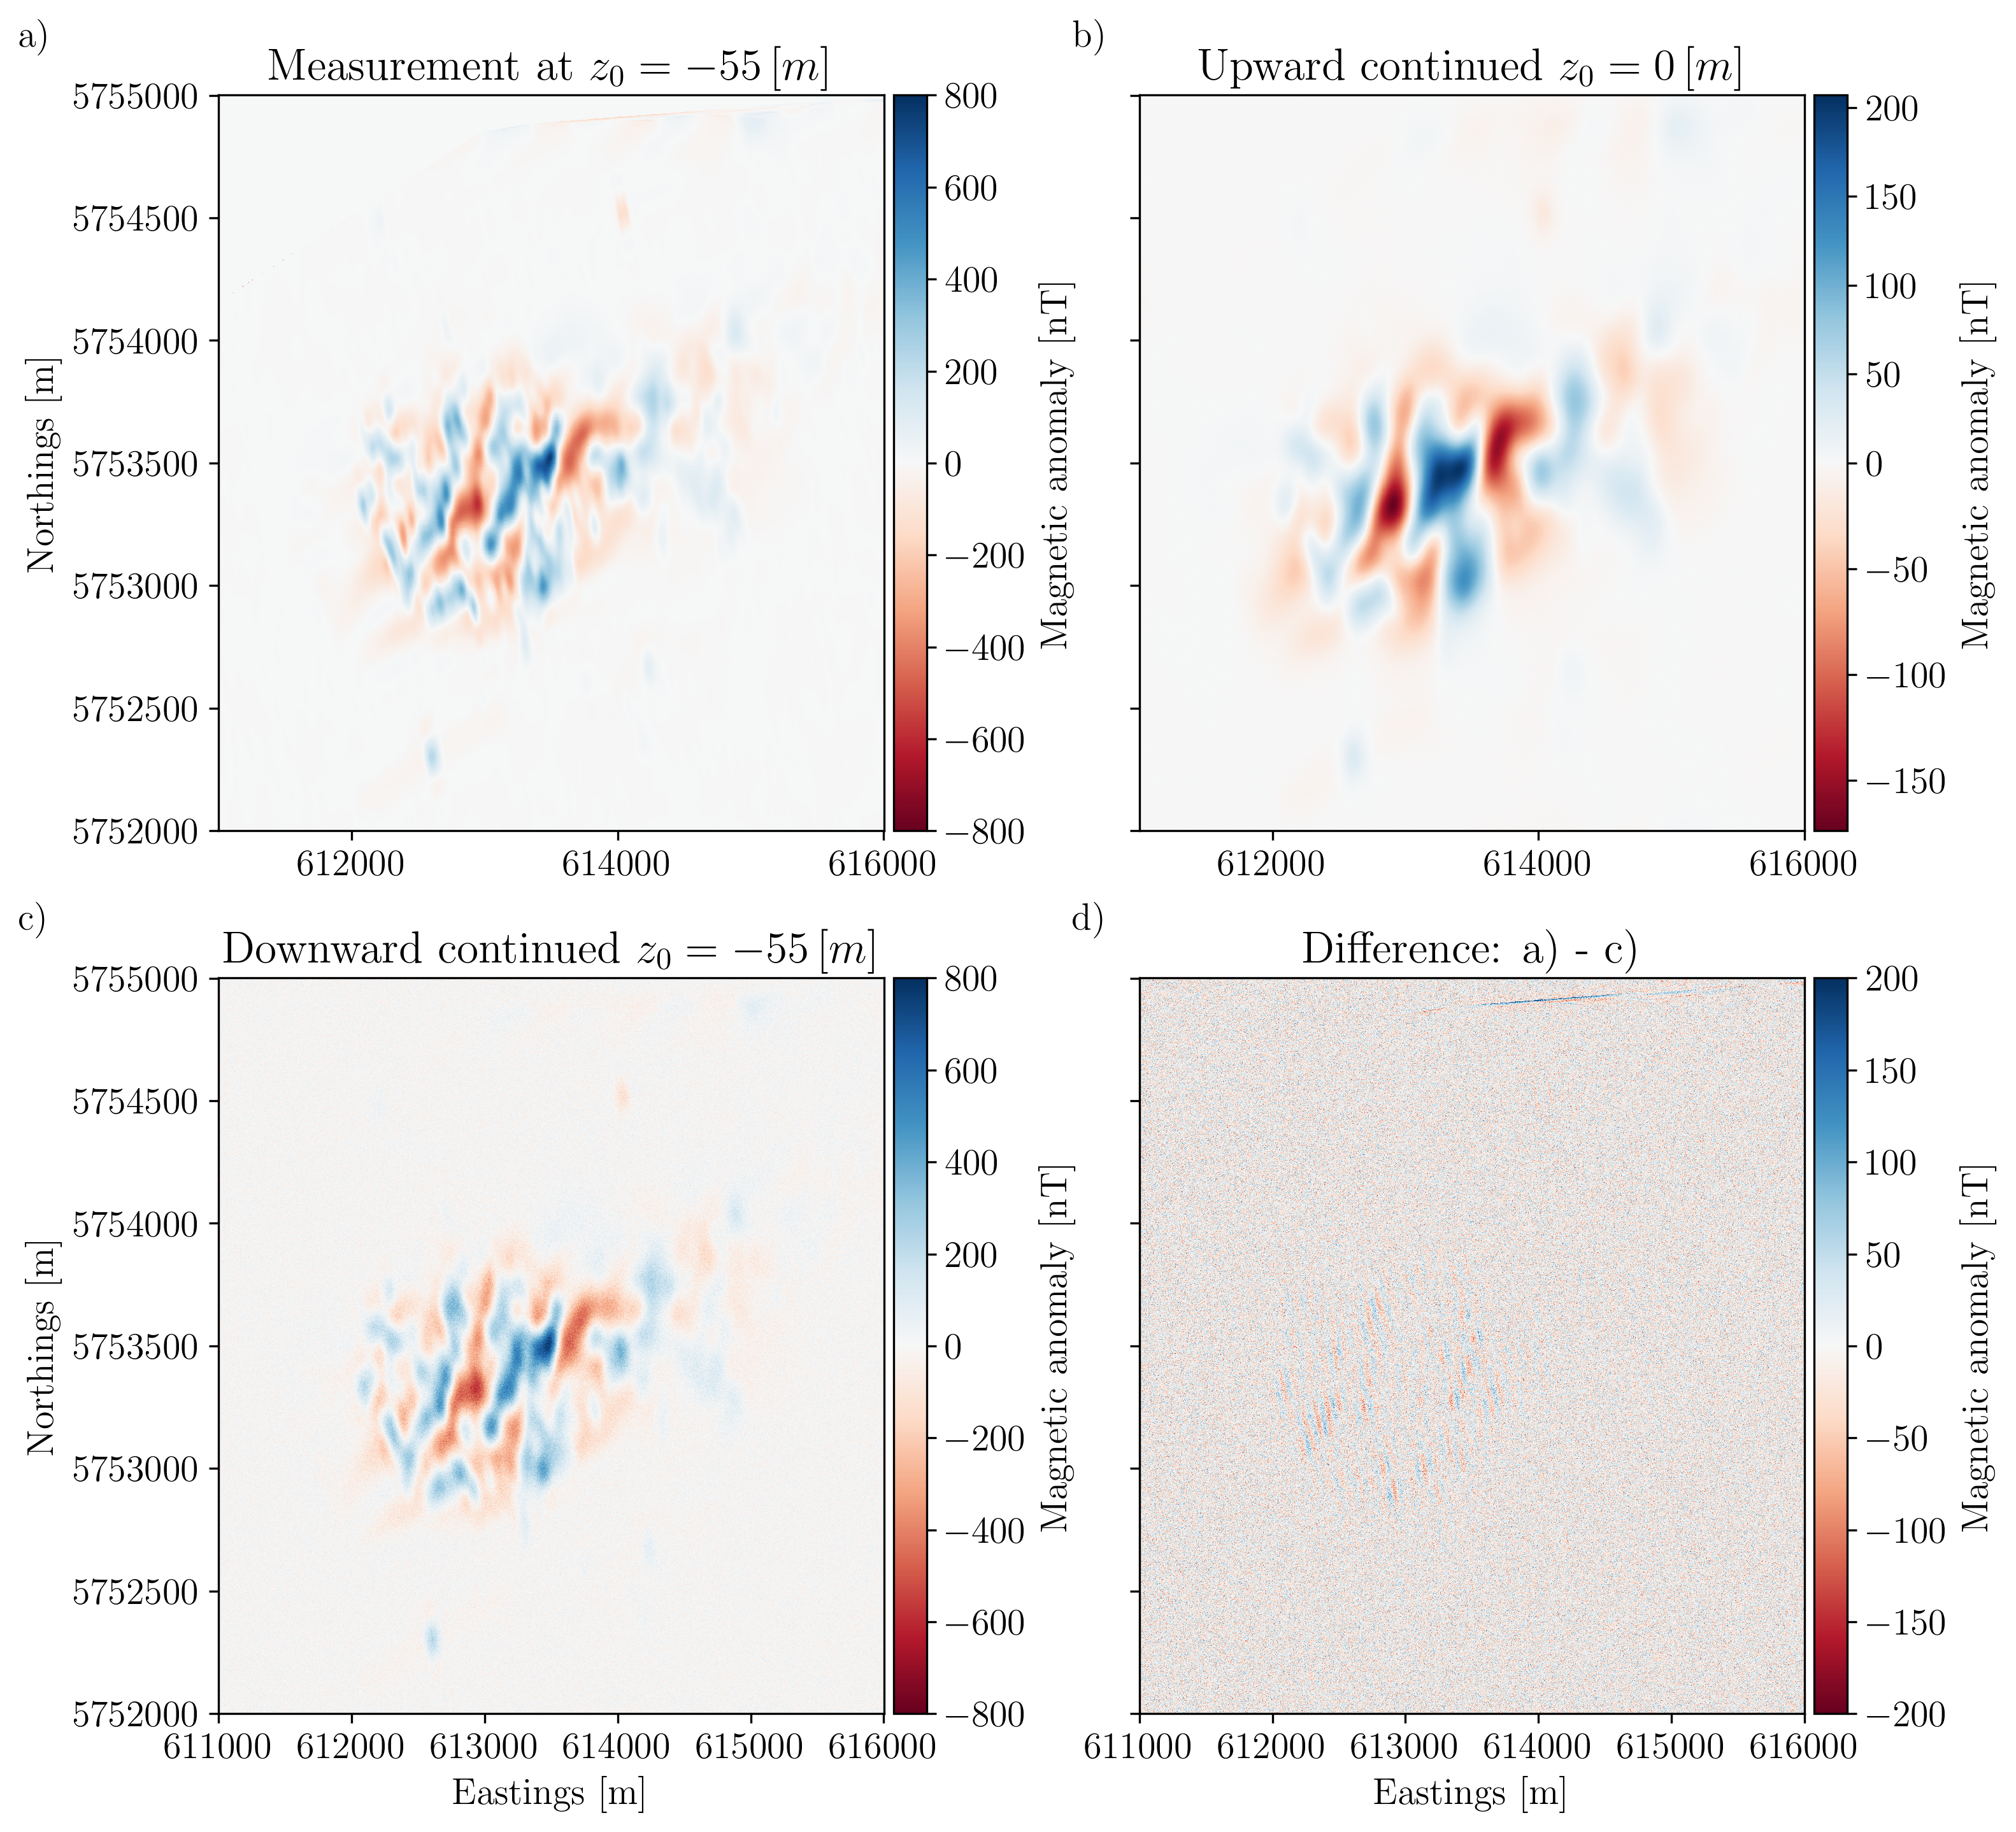
\includegraphics[width=0.9\textwidth]{./figs/compare_residuals_V3_noise1.0.png}
	\caption{\fb
		a) displays the cubic interpolated measured field at an altitude of 5[m] which is -55[m] below the surface.
		b) displays the upward continued field of a) {\bf perturbed} with additive white noise $\mathcal{N}(0,1.0\,\text{[nT]})$.
		c) displays the downward continued field of b) using 20 iterations.
		d) displays the absolute error between the estimated field in c) and the measured one in a).
		The corresponding decreasing RMSE is depicted in Fig.~\ref{fig:green_20sig1rmse}.
	}
	\label{fig:green_20sig1}
\end{figure*}

\begin{figure}
	\centering
	\includegraphics[width=0.9\columnwidth]{./figs/rmse_residuals_V3_noise1.0.png}
	\caption{\fb
		The reconstruction RMSE of downward continuing additive white noise $\mathcal{N}(0,1.0\,\text{[nT]})$ whose result is depicted in Fig.~\ref{fig:green_20sig1}.
	}
	\label{fig:green_20sig1rmse}
\end{figure}

\begin{figure*}
	\centering
	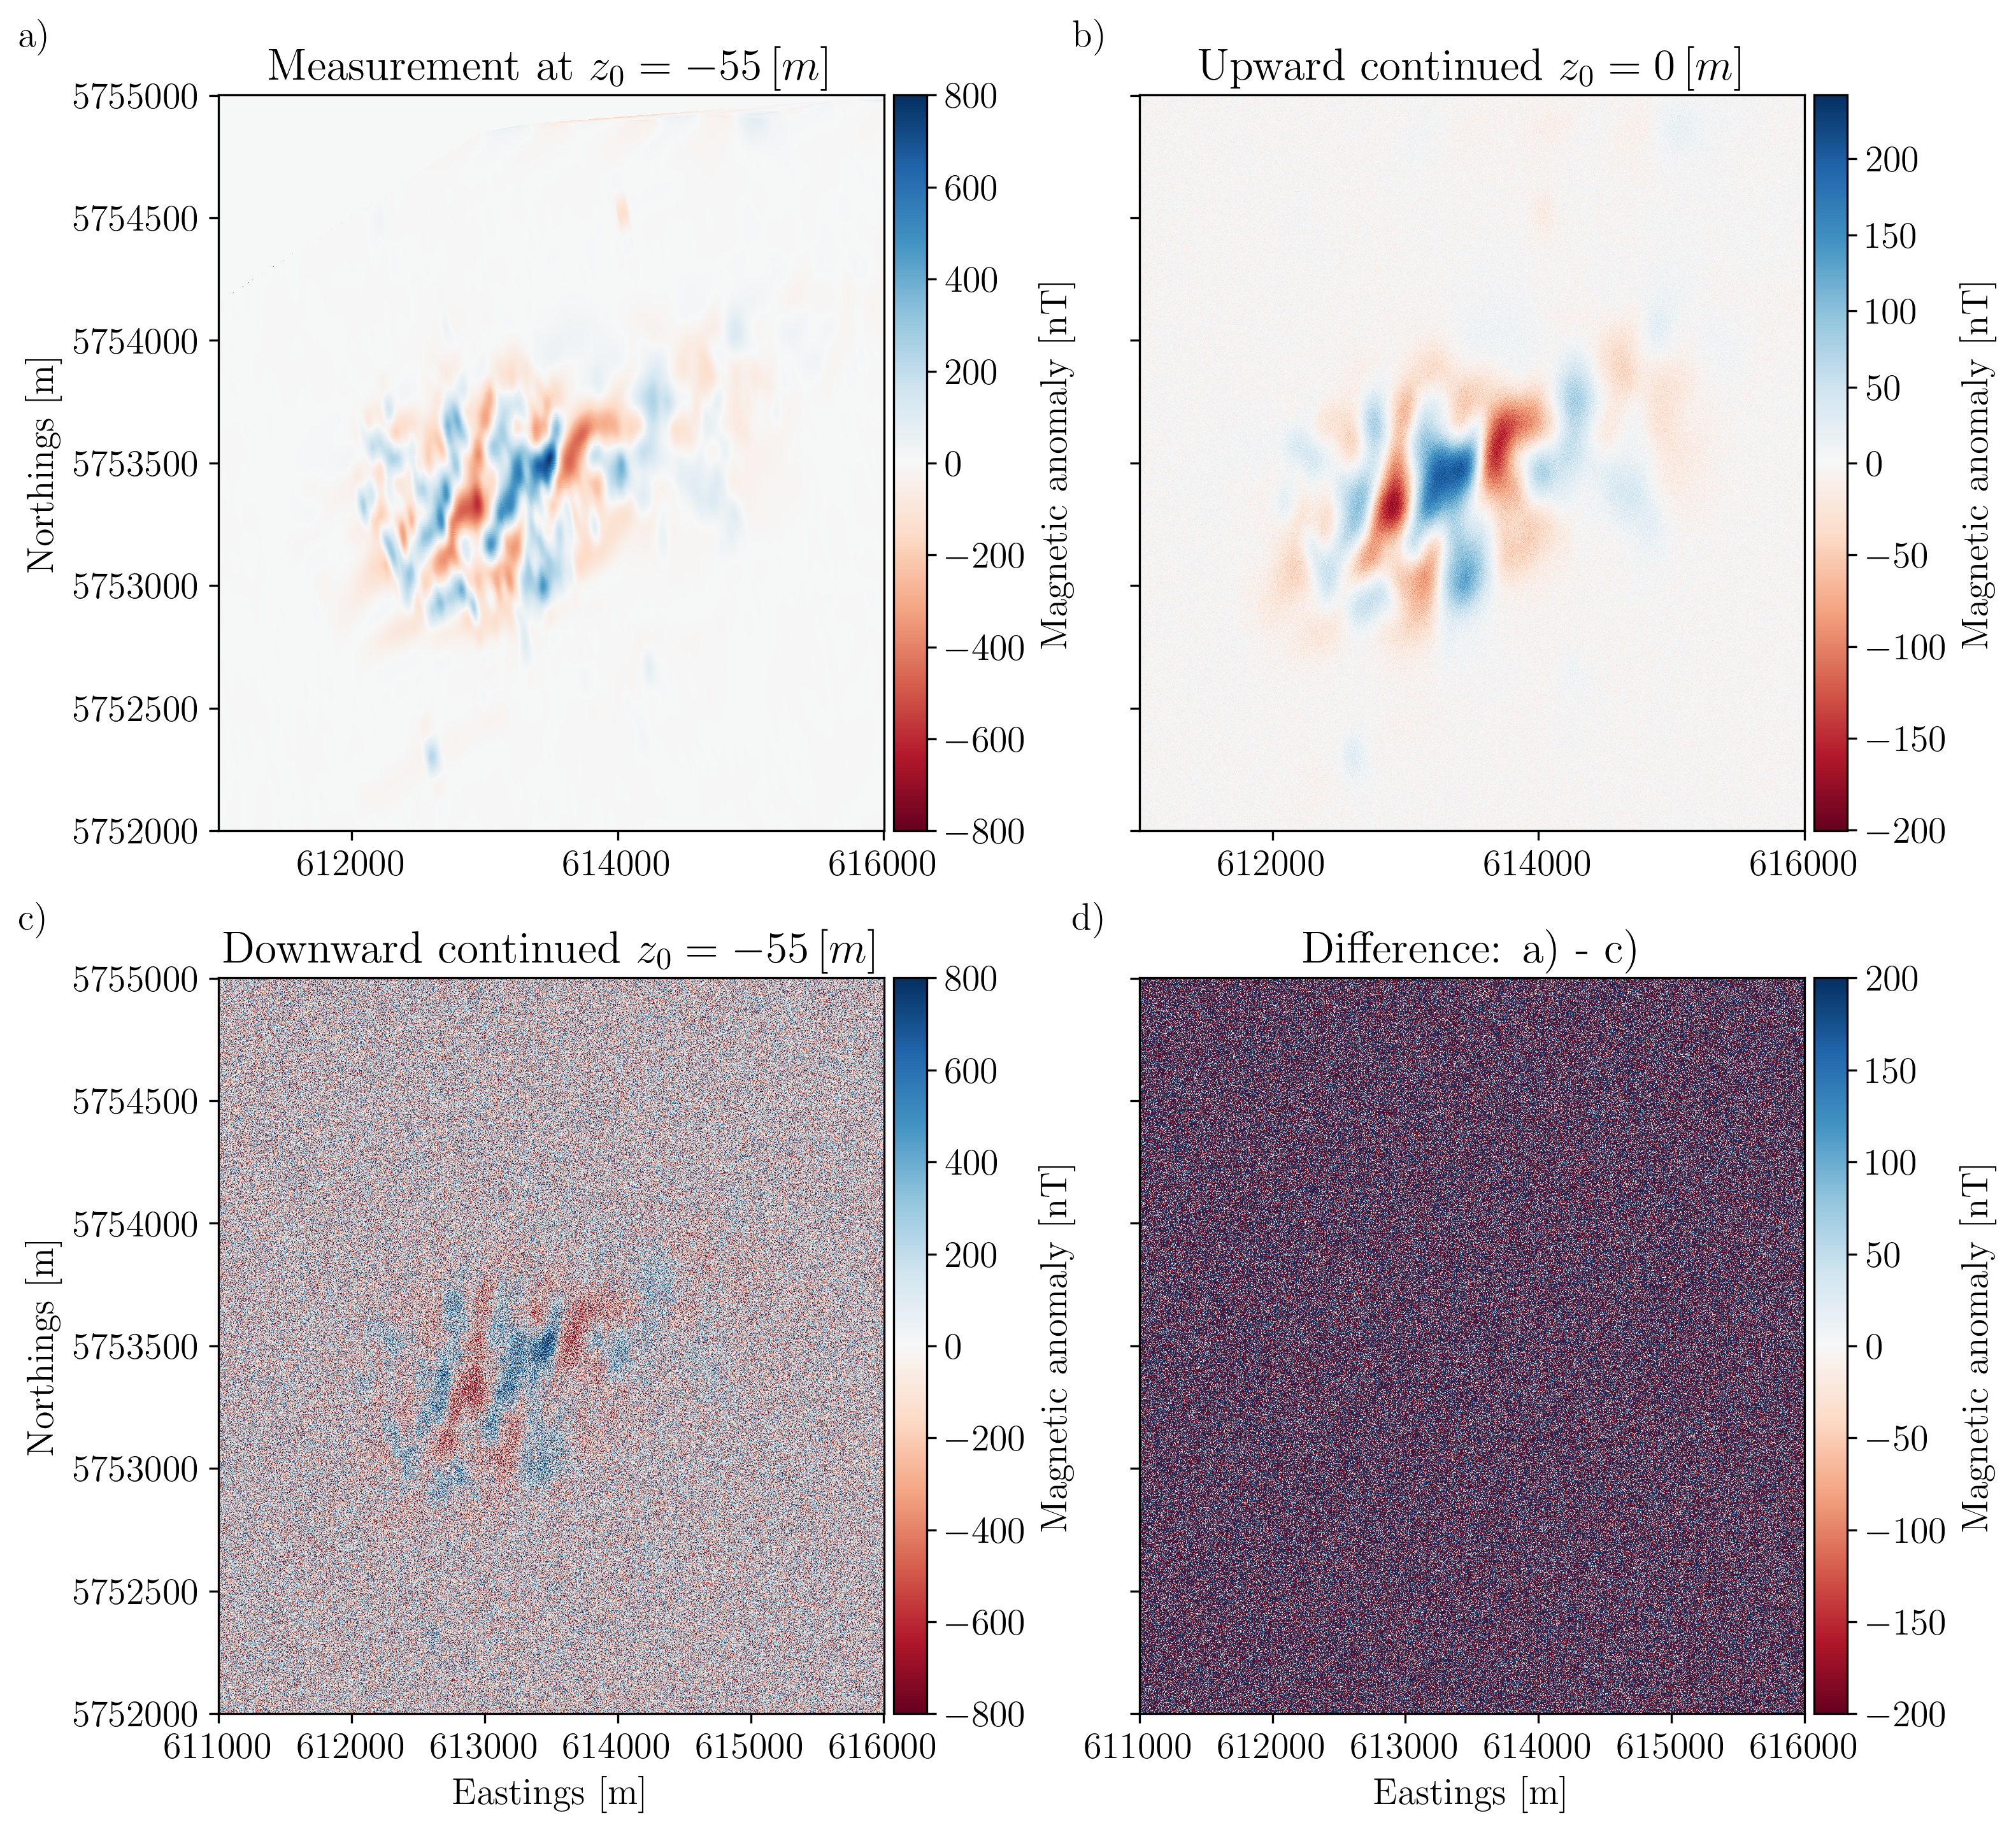
\includegraphics[width=0.9\textwidth]{./figs/compare_residuals_V3_noise10.0.png}
	\caption{\fb
		a) displays the cubic interpolated measured field at an altitude of 5[m] which is -55[m] below the surface.
		b) displays the upward continued field of a) {\bf perturbed} with additive white noise $\mathcal{N}(0,10.0\,\text{[nT]})$.
		c) displays the downward continued field of b) using 20 iterations.
		d) displays the absolute error between the estimated field in c) and the measured one in a).
		The corresponding decreasing RMSE is depicted in Fig.~\ref{fig:green_20sig10rmse}.
	}
	\label{fig:green_20sig10}
\end{figure*}

\begin{figure}
	\centering
	\includegraphics[width=0.9\columnwidth]{./figs/rmse_residuals_V3_noise10.0.png}
	\caption{\fb
		The reconstruction RMSE of downward continuing additive white noise $\mathcal{N}(0,1.0\,\text{[nT]})$ whose result is depicted in Fig.~\ref{fig:green_20sig10}.
	}
	\label{fig:green_20sig10rmse}
\end{figure}







\subsection{INFOMAR}


{\fb
Here, we apply out method on data acquired by \verb|CV_13_01|.
First, we grid the raw measurements similar to section~\ref{sec:green_rebel}.
However, due to the quality of the data that is a lens dense survey lines and non-readable file, we could only apply a linear interpolation since a cubic yielded a non-stable result.
The estimated field at the surface is depicted in Fig.~\ref{fig:case_study} b).
Moreover, we note the associated artifacts caused by the linear interpolation and more importantly the qualitative difference to the upward continued Green rebel data (see Fig.~\ref{fig:case_study} b) ).

Given this limitation, we only qualitatively investigate the performance of the algorithm.
The estimated downward field of \verb|CV_13_01|, after three iterations, is depicted in Fig.~\ref{fig:case_study} a).
Comparing it with the measured field by Green rebel (Fig.~\ref{fig:case_study} a) and c) ) shows that the order of magnitude of the magnetic anomaly map matches and the rough geological location given the limitation that the upward field already heavily disagreed (Fig.~\ref{fig:case_study} f)).

\todo{maybe to compare: redo Tikhonov regularization and show that it does not work for SeaLink data}

%The magnetic anomalies at the sea level and and the seabed are displayed in Fig.~\ref{fig:case_study} b) and c).
%The region features a large geographic magnetic anomaly whose magnitude ranges from 
%and a small one cause by an unidentified ship wreck~\cite{infomar_shipwreck}, whose location is marked green in Fig.~\ref{fig:case_study}.
%Due magnitude of the geographic anomaly the 

%The magnetic anomaly measured at the surface is shown in Fig.~\ref{fig:case_study} b) and will be denoted $U(x,y,0)$.



\begin{figure}
	\centering
	\includegraphics[width=.9\columnwidth]{./figs/wreck_1D_infomar.png}
	\caption{
		At $51.92951\degree$ N, $-7.34118\degree$ W is an unidentified ship wreck~\cite{infomar_shipwreck}.
	}
	\label{fig:wreck_infomar}
\end{figure}



Accordingly, the measured anomaly close to the seabed is shown in Fig.~\ref{fig:case_study} c), will be denoted $\hat{U}(x,y,-55)$.

We start with the numerical stable upward continuation and use Eq.~\eqref{eq:inverseFourierTransfor} to obtain $\hat{U}(x,y,0)$ (shown in Fig.\ref{fig:case_study} c) ).
         

}





\begin{figure*}
	\centering
	\includegraphics[width=0.9\textwidth]{./figs/compare_residuals_V2.png}
	\caption{\fb
		The area survey by CV\_13\_01 features a large geographic magnetic anomaly and a small one caused by an unidentified wreck whose location is marked in green~\cite{infomar_shipwreck}.
		The anomalies are measured both at the surface and close to the seabed and up and downward continued accordingly.
		a) shows the downward continued field at $z_0=-55\,[m]$ of the field obtained by INFOMAR at the surface at $z_0=0\,[m]$.
		b) shows the field obtained by INFOMAR at the surface at $z_0=0\,[m]$.
		c) shows the field obtained by Green rebel close to the seabed at $z_0=5\,[m]$.
		d) shows the upward continued field at $z_0=0\,[m]$ of the field obtained by Green rebel close to the seabed at $z_0=5\,[m]$.
		e) shows the difference between the estimated field of a) and the measured field in c).
		f) shows the difference between the estimated field in d) and the measured field in b).
	}
	\label{fig:case_greenRebel_Sealink}
\end{figure*}



\section{Own data measured at different altitudes}



\section{Conclusion}

Here, we presented an open source software that enables end-user to process Infomar's magnetometry data and export anomaly grids for further investigation.
%The processing includes a reading, cleaning and gridding of the data and an optional downward continuation to the seabed.
%Next steps include the ground truthing of selected anomalies to further improve the downward continuation and to enable the full potential of this rich data set.




% Numbered list
% Use the style of numbering in square brackets.
% If nothing is used, default style will be taken.
%\begin{enumerate}[a)]
%\item 
%\item 
%\item 
%\end{enumerate}  

% Unnumbered list
%\begin{itemize}
%\item 
%\item 
%\item 
%\end{itemize}  

% Description list
%\begin{description}
%\item[]
%\item[] 
%\item[] 
%\end{description}  

% \clearpage %%Remove this from your manuscript

% % Figure
% \begin{figure}%[]
%   \centering
% %    \includegraphics{}
%     \caption{}\label{fig1}
% \end{figure}


% \begin{table}%[]
% \caption{}\label{tbl1}
% \begin{tabular*}{\tblwidth}{@{}LL@{}}
% \toprule
%   &  \\ % Table header row
% \midrule
%  & \\
%  & \\
%  & \\
%  & \\
% \bottomrule
% \end{tabular*}
% \end{table}

% Uncomment and use as the case may be
%\begin{theorem} 
%\end{theorem}

% Uncomment and use as the case may be
%\begin{lemma} 
%\end{lemma}

%% The Appendices part is started with the command \appendix;
%% appendix sections are then done as normal sections
%% \appendix

%\section{}\label{}

% To print the credit authorship contribution details
\printcredits

%% Loading bibliography style file
%\bibliographystyle{model1-num-names}
\bibliographystyle{cas-model2-names}

% Loading bibliography database
\bibliography{cas-refs}

% Biography
%\bio{}
% Here goes the biography details.
%\endbio

%\bio{pic1}
% Here goes the biography details.
%\endbio

\end{document}

